% Modultest fugt og temp print

%tekst

I følgende afsnit testes fugt- og temperatursensoren sammen med lavpasfilter på det færdigudarbejdet PCB. Der testes for om temperatur og fugtighedsændringer registreres korrekt og om omregningen fra DC-niveau til værdi stemmer overens med scenariet i test. Scopbillederne er taget med et agilent oscilloskop.

SHT21p-sensoren udsender et PWM-signal med en frekvens på 120 hz i området 0V til VCC. Ud fra PWMen kan temperatur og fugtighed udregnes med følgende formler som er hentet fra databladet:

\begin{equation}
-6+125*duty cycle= fugtighed \ i \ \%
\end{equation}

\begin{equation}
-46.85+175.72*duty cycle= temperatur \ i \ grader \ celsius
\end{equation}

PWM-signalet bliver, gennem et 2. ordens lavpasfilter, midlet til en DC. Ud fra denne DC-
og VCC-værdi beregnes fugtigheden og temperaturen ved følgende formler.


\begin{equation}
-6+125*\frac{målt DC}{Vcc}= fugtighed \ i \ \%
\end{equation}

\begin{equation}
-46.85+175.72*\frac{målt DC}{Vcc}=temperatur \ i \ grader \ celsius
\end{equation}

Sensoren er forsynet med 3,3V men grundet et lille tab i sensoren svinger PWMen mellem
0 og 3,28 V.


%Billede af målt PWM.


Første test laves ved stuetemperatur. Til test af SHT21p sensoren bruges et færdigt termometer og fugtighedsmåler, af modellen Velleman - Thermo/Hygrometer. På figur \ref{lab:TEST_STUE} ses det at begge sensorer er i samme rum og at de bliver udsat for samme forhold. 

\begin{figure}[H] \centering
\begin{minipage}[b]{0.48\textwidth} \centering
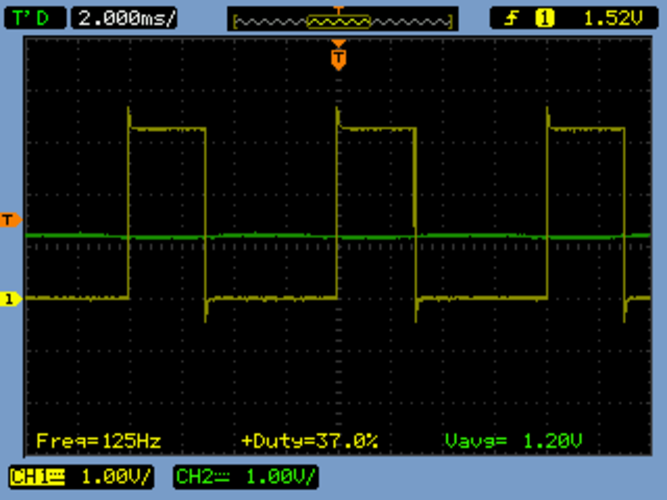
\includegraphics[width=1.00\textwidth]{filer/modultest/Billeder/SCOP_humidSTUETEMP} % Left picture
\end{minipage} \hfill
\begin{minipage}[b]{0.48\textwidth} \centering
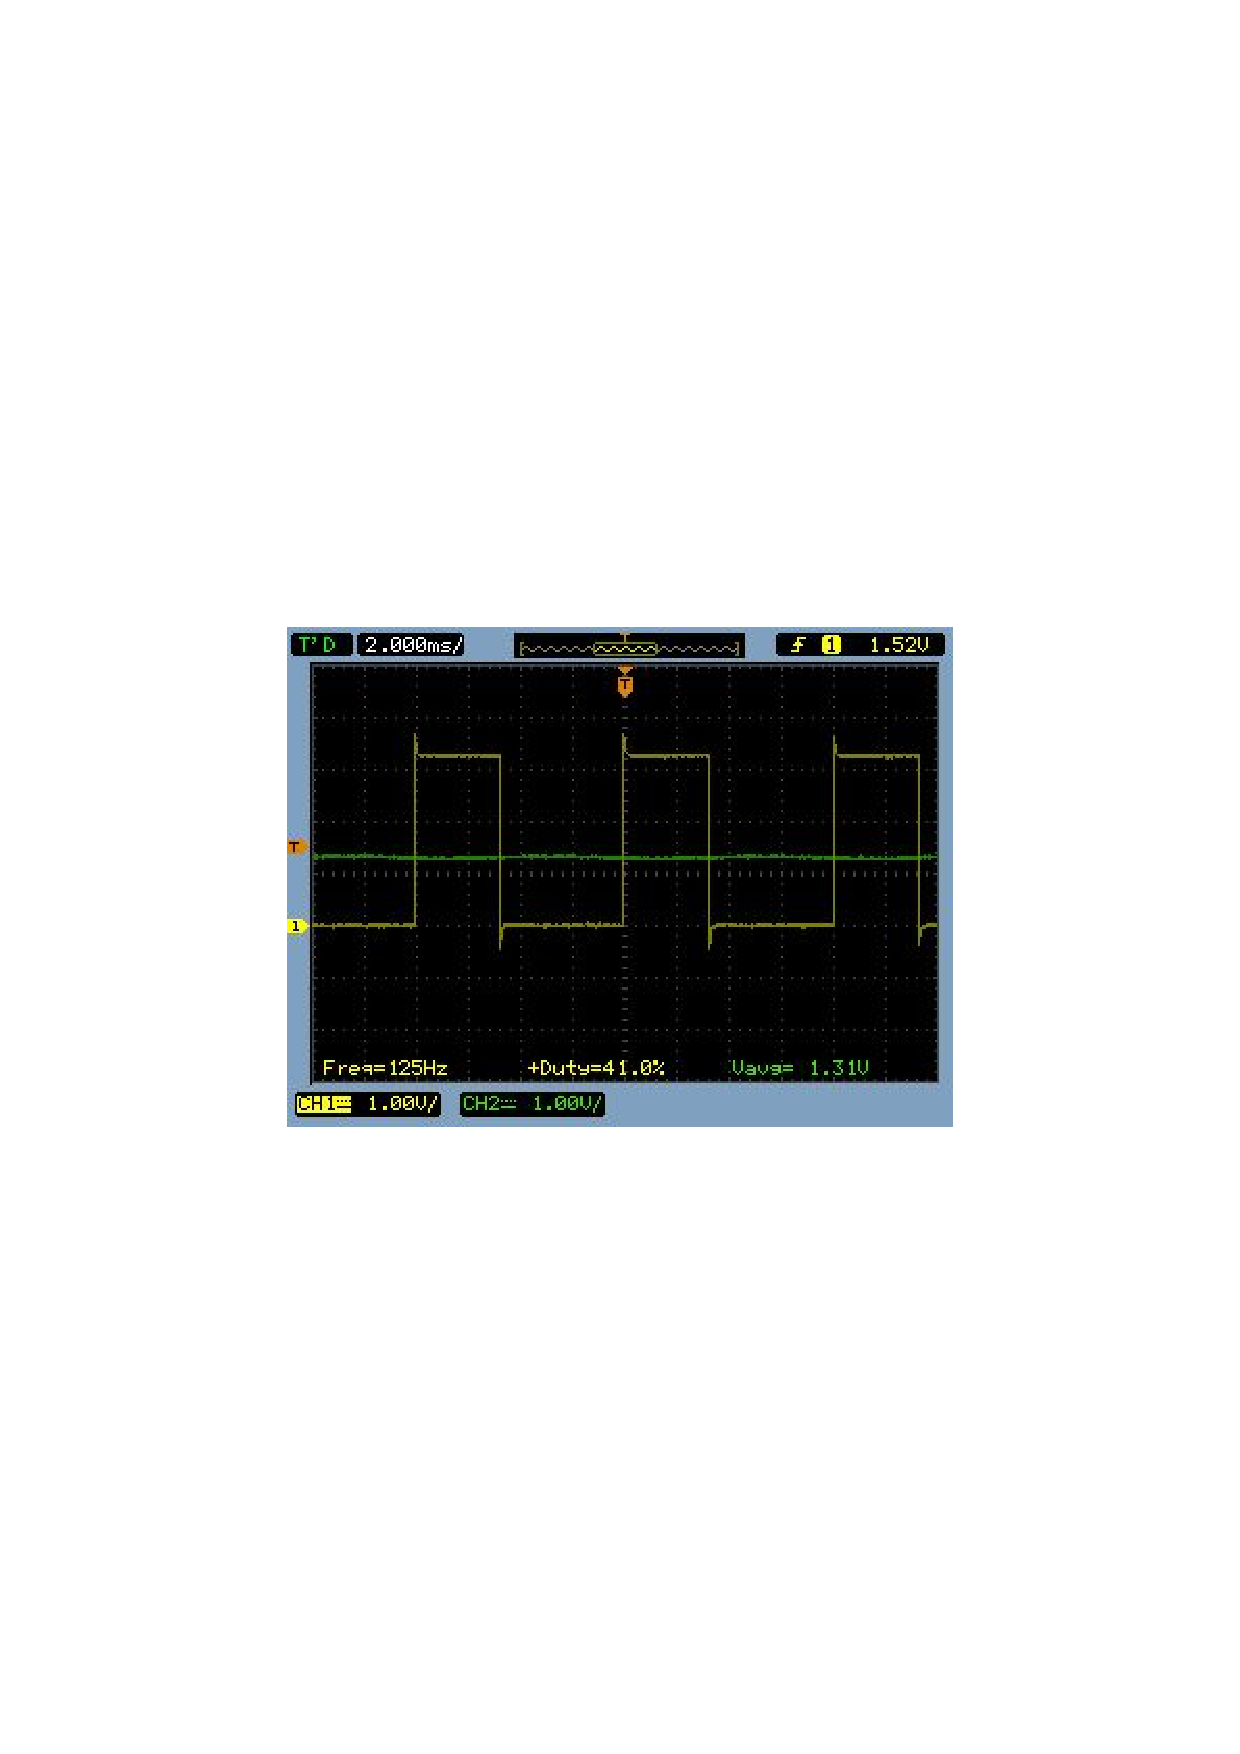
\includegraphics[width=1.00\textwidth]{filer/modultest/Billeder/SCOP_tempSTUETEMP} % Right picture
\end{minipage} \\ % Captions og labels
\begin{minipage}[t]{0.48\textwidth}
\caption{Oscilloskopbillede af fugthedsmåling ved stuetemperatur} % Left caption and label
\label{fig:SCOP_FUGT_STUE}
\end{minipage} \hfill
\begin{minipage}[t]{0.48\textwidth}
\caption{Oscilloskopbillede af temperaturmåling ved stuetemperatur} % Right caption and label
\label{fig:SCOP_TEMP_STUE}
\end{minipage}
\end{figure}

\begin{figure}[H]
\centering
{\includegraphics[width=0.90\textwidth]{filer/modultest/Billeder/test_STUE}}
\caption{Billede af test ved stuetemperatur}
\label{lab:TEST_STUE}
\end{figure}



Som figur \ref{fig:SCOP_FUGT_STUE} viser måles både en DC- og et PWM-signal. DCen er signalet efter lavpasfilteret og PWMen er den rå data fra sensoren. 
Sensorens SCL-ben er sat højt, via pull-up-modstanden på sensorprintet, sensoren måler derfor fugtighed. PWMen måles til at have en duty cycle på 37 \% og spændingen efter filteret måles til 1,2 V. Ud fra databladet kan duty cyclen omregnes til fugtighed med følgende formel:

Fugtighed regnet ud fra duty cycle
\begin{equation}
-6+125*0.37=40,25\%
\end{equation}

Med følende formel regnes fugtigheden ud fra DC-værdien.
\begin{equation}
-6+125*\frac{1,2}{3,28}= 39,73\%
\end{equation}

SCL-benet ligges nu lav, ved at forbinde benet til GND, og temperaturen måles. Figur \ref{fig:SCOP_TEMP_STUE} viser målingen. PWMen måles til at have en duty cycle på 41 \% og en spænding efter filteret på 1.31 V. 
Ud fra PWMen regnes nu temperaturen.
\begin{equation}
-46.85+175.72*0,41=25.2^{\circ}C
\end{equation}

Temperaturen regnes ud fra DCen som følger. 

\begin{equation}
-46.85+175.72*\frac{1,31}{3,28}=23.33^{\circ}C
\end{equation}


For at teste andre forhold bruges en varmepistol til at hæve temperatur og sænke fugtigheden, figur \ref{lab:TEST_VARM}. 
Samme målinger foretages:


\begin{figure}[H] \centering
\begin{minipage}[b]{0.48\textwidth} \centering
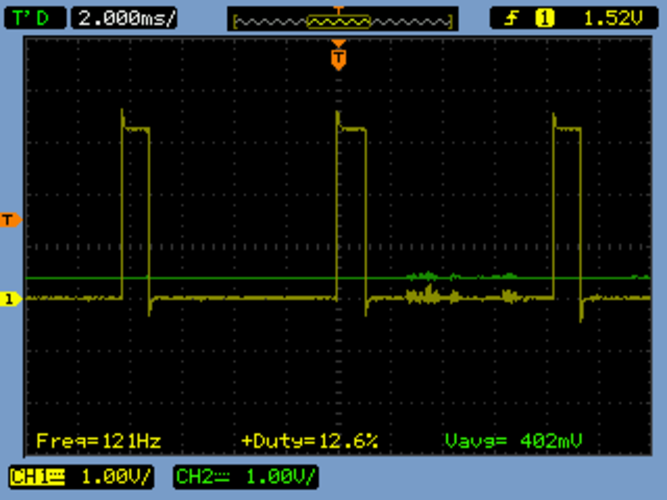
\includegraphics[width=1.00\textwidth]{filer/modultest/Billeder/SCOP_humidVARM} % Left picture
\end{minipage} \hfill
\begin{minipage}[b]{0.48\textwidth} \centering
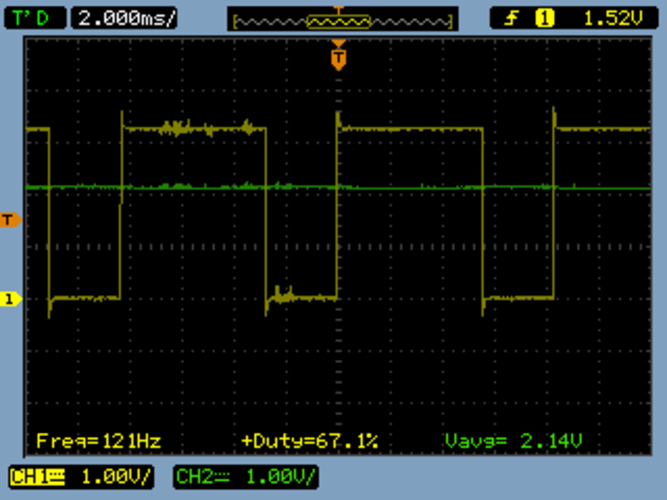
\includegraphics[width=1.00\textwidth]{filer/modultest/Billeder/SCOP_tempVARM} % Right picture
\end{minipage} \\ % Captions og labels
\begin{minipage}[t]{0.48\textwidth}
\caption{Oscilloskopbillede af fugthedsmåling ved høj temperatur} % Left caption and label
\label{fig:SCOP_FUGT_VARM}
\end{minipage} \hfill
\begin{minipage}[t]{0.48\textwidth}
\caption{Oscilloskopbillede af temperaturmåling ved høj temperatur} % Right caption and label
\label{fig:SCOP_TEMP_VARM}
\end{minipage}
\end{figure}

\begin{figure}[H]
\centering
{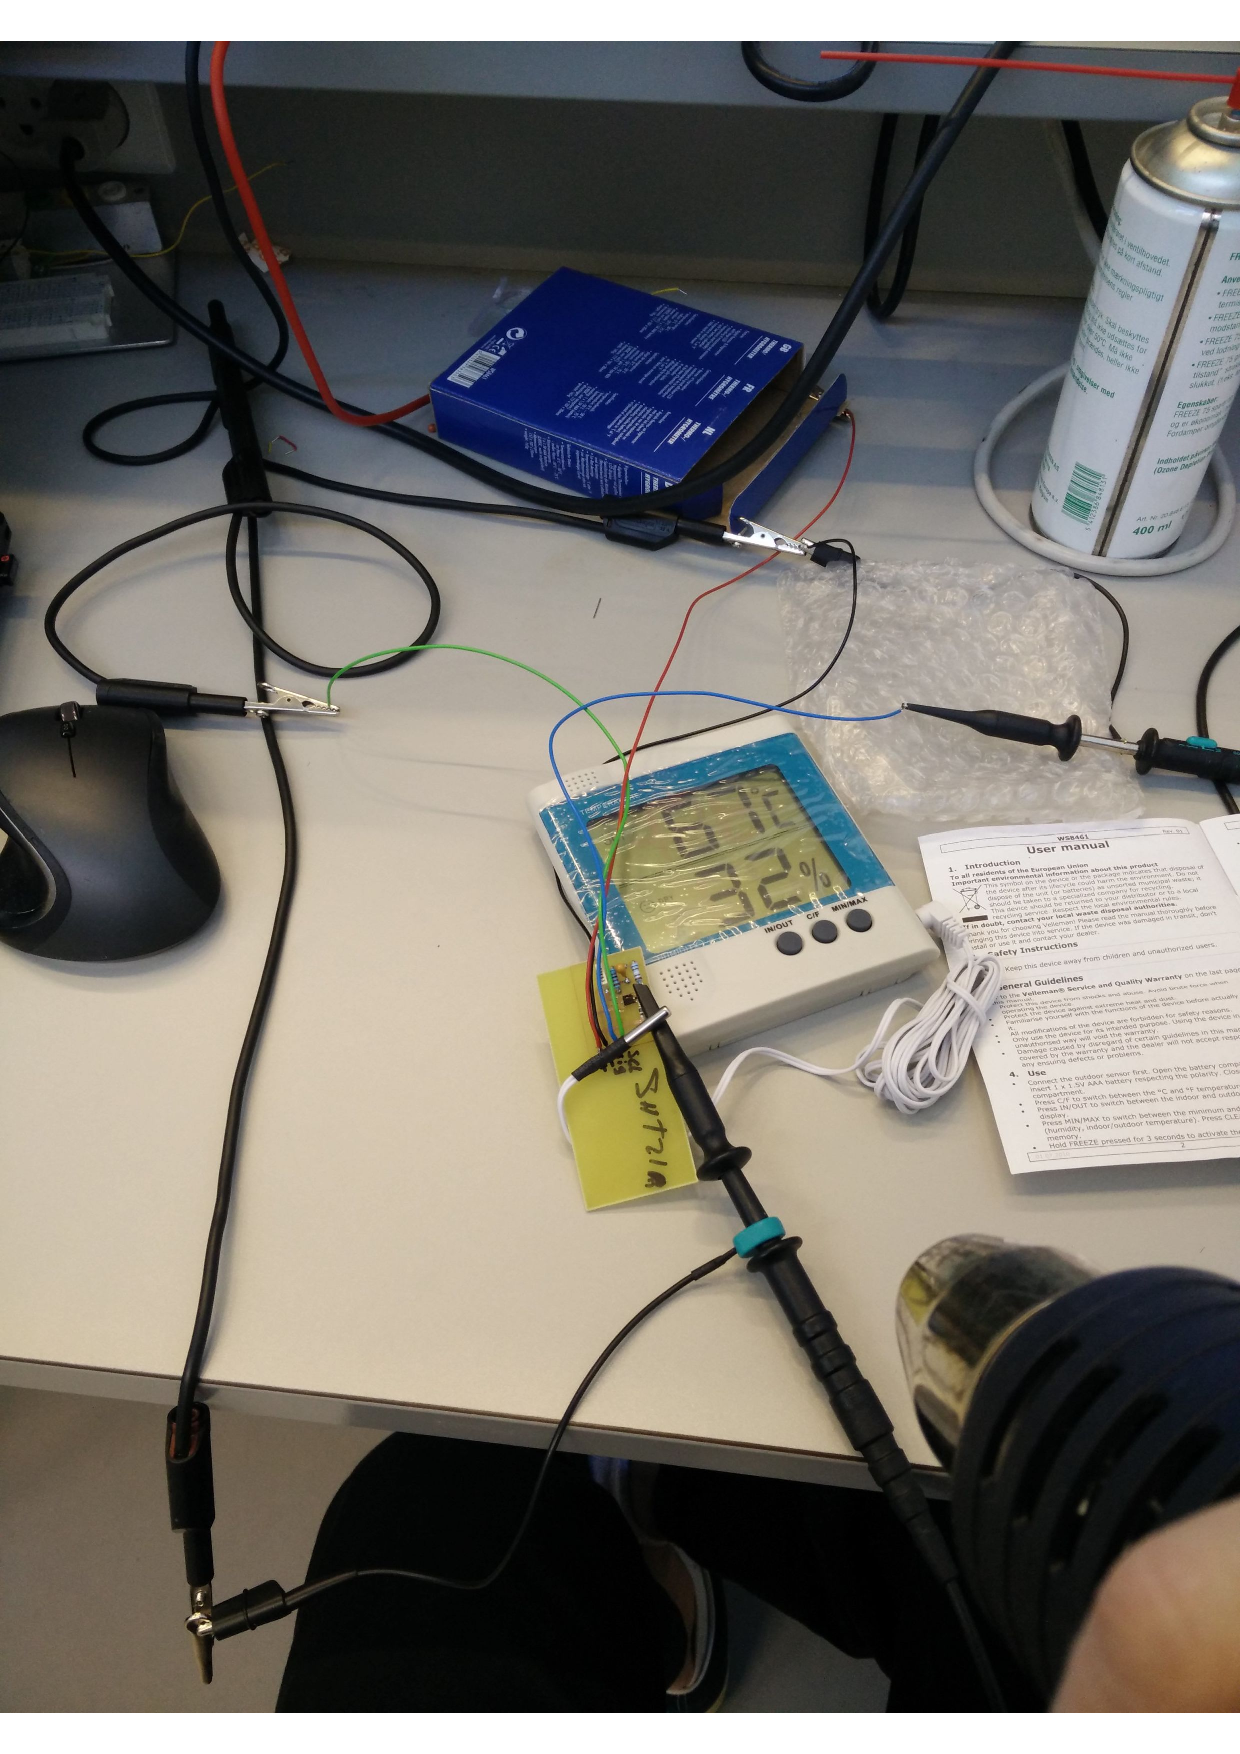
\includegraphics[width=0.90\textwidth]{filer/modultest/Billeder/test_VARM}}
\caption{Billede af test ved høj temperatur}
\label{lab:TEST_VARM}
\end{figure}

Igen regnes værdierne for temperatur og fugtighed ud fra PWMen med en dutycycle på 12,6 \% og DCen med en amplitude på 402 mV, målt som vist på figur \ref{fig:SCOP_FUGT_VARM}.

\begin{equation}
-6+125*0,126= 9,75\%
\end{equation}

Med følgende formel regnes fugtigheden ud fra DC-værdien.

\begin{equation}
-6+125*\frac{0,402}{3,28}= 9,32\%
\end{equation}

SCL-benet sættes nu lavt ved at forbinde det til GND og temperaturen måles. Sensoren giver en PWM på 67,1 \% og en spænding efter filteret på 2,14 V, målt som vist på \ref{fig:SCOP_TEMP_VARM}. 
Ud fra PWM beregnes temperaturen.


\begin{equation}
-46.85+175.72*0,671=71,06^{\circ}C
\end{equation}

Temperaturen regnes ud fra DCen som følger. 

\begin{equation}
-46.85+175.72*\frac{1,31}{3,28}=67,8^{\circ}C
\end{equation}

For også at teste om sensoren kunne måle en høj luftfugtig foretages en måling efter at have åndet på sensoren, målingen ses på figur \ref{lab:TEST_FUGTIG}. Da der allerede er målt temperatur ved både stuetemperatur og høj temperatur udelades temperaturtest af denne test. 

\begin{figure}[H]
\centering
{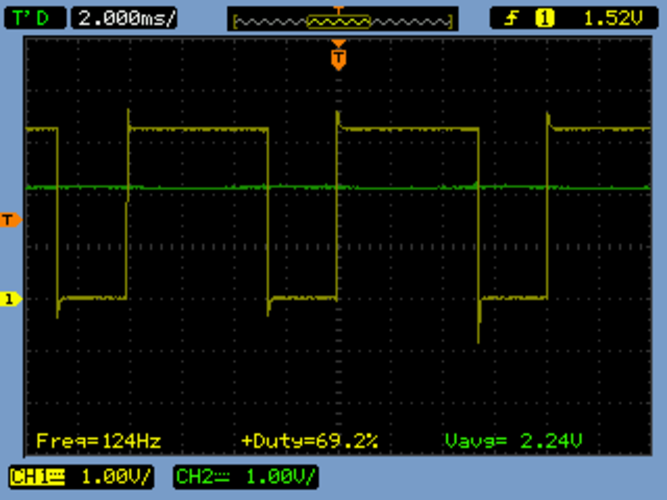
\includegraphics[width=0.90\textwidth]{filer/modultest/Billeder/SCOP_humidFUGTIG}}
\caption{Oscilloskopbillede af fugtighedsmåling med høj luftfugtighed}
\label{lab:SCOP_FUGT_FUGTIG}
\end{figure}

\begin{figure}[H]
\centering
{\includegraphics[width=0.90\textwidth]{filer/modultest/Billeder/test_FUGTIG}}
\caption{Oscilloskopbillede af fugtighedsmåling med høj luftfugtighed}
\label{lab:TEST_FUGTIG}
\end{figure}


Ved testen sendte sensoren en PWM ud med en duty cycle på 69,2 \% og en spænding på 2,24 V efter filteret, oscilloskopbillede ses på figur \ref{lab:SCOP_FUGT_FUGTIG}.


\begin{equation}
-6+125*0,692= 80,5\%
\end{equation}

Med følgende formel regnes fugtigheden ud fra DC-værdien.

\begin{equation}
-6+125*\frac{2,24}{3,28}= 79,37\%
\end{equation}


En test ved lav temperatur blev også fortaget. Temperaturen blev sænket ved hjælp af frysespray, se figur \ref{lab:TEST_KOLD}. Grundet den lave temperatur opstod der kondensvand på sensoren, derfor er fugtighed udeladt af denne måling.


\begin{figure}[H]
\centering
{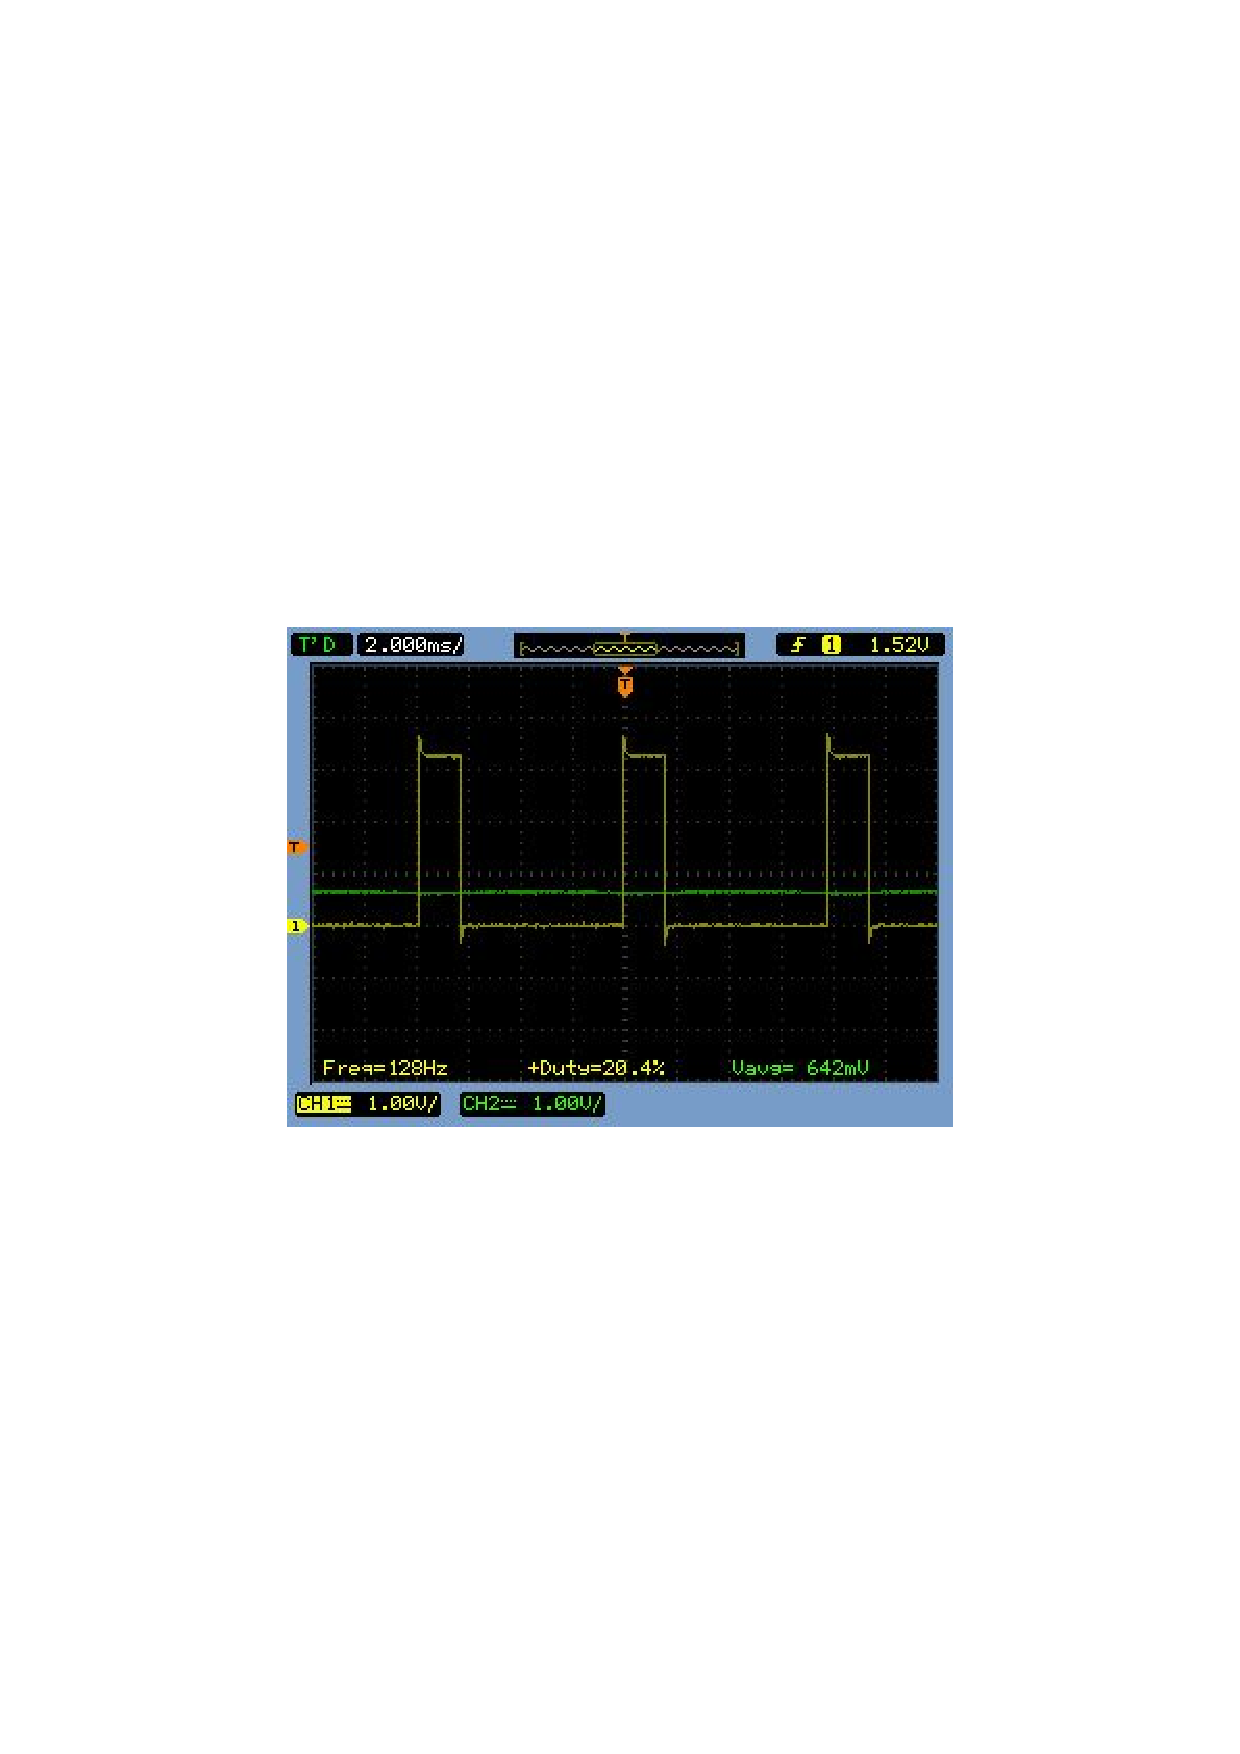
\includegraphics[width=0.90\textwidth]{filer/modultest/Billeder/SCOP_tempKOLD}}
\caption{Oscilloskopbillede af fugtighedsmåling med høj luftfugtighed}
\label{lab:SCOP_TEMP_KOLD}
\end{figure}

\begin{figure}[H]
\centering
{\includegraphics[width=0.90\textwidth]{filer/modultest/Billeder/test_KOLD}}
\caption{Oscilloskopbillede af fugtighedsmåling med høj luftfugtighed}
\label{lab:TEST_KOLD}
\end{figure}

Sensoren giver en PWM på 20,4 \% og en spænding efter filteret på 642 mV,se figur\ref{lab:SCOP_TEMP_KOLD}. Temperatur beregnes herefter.


\begin{equation}
-46.85+175.72*0,204=-11^{\circ}C
\end{equation}

Temperaturen regnes ud fra DCen. 

\begin{equation}
-46.85+175.72*\frac{0,642}{3,28}=-12,66^{\circ}C
\end{equation}


Testen viser at fugtighedsmålingerne passer meget godt overens når man sammenligner målingen af det velleman hygrometeret, den rå PWM fra sensoren og den midlede DC efter filteret. Temperaturmålingerne er dog ligger dog lidt lavere efter filteret end hvis man regner værdierne med PWMen. Denne forskel kan skyldes at filteret belaster sensoren en smule eller at målingen kan have været upræcis. Det ses at målingerne lavet med SHT21p og Velleman stemmer nogenlunde overens. Da Velleman termo- hygrometeret reagerede meget langsomt på ændringer godtages det at der er afvigelser mellem målingerne lavet af Velleman og SHT21p. 

